\documentclass{article}
\usepackage[letterpaper,margin=1.0in]{geometry}
\usepackage{setspace}
\usepackage[pdftex]{graphicx}
\begin{document}
\title{Knowledge Advantage Desktop: Interface, Infrastructure, and Markup}
\author{Larry Reaves}
\maketitle
\pagebreak
\begin{doublespace}
\section{Introduction}
In modern times, we are inundated with a huge amount of information for a wide range of sources.
While making sense of this fire hose of knowledge can be quite a challenge, it is essential to be able
to function in many of today's work environments.
Knowledge Advantage Desktop (KAD) is a tool for discovering information, extracting meaning,
finding connections between different pieces of information,
and visualizing the knowledge that has been processed.
\par
By leveraging KAD, a knowledge worker is able to more quickly find information that is relevant to their
work by inputting search parameters.
After the software finds a piece of information matching the search parameters,
it will extract important words from the text as well as other information such as the author or date of publication.
Combined, the document and these annotations make up what we call a JAN.
These JANs are then networked by finding common metadata such as keywords or authors.
This network is visualized so that the user can easily move from one document to related documents.
The network can also be searched to find a particular keyword or author.
\par
A group of networked JANs is called a JANBase.
KAD supports the ability to switch between JANBases so that you can have separate networks for different topics.
This makes it easier to find information relevant to your current work objective.
\section{Interface}
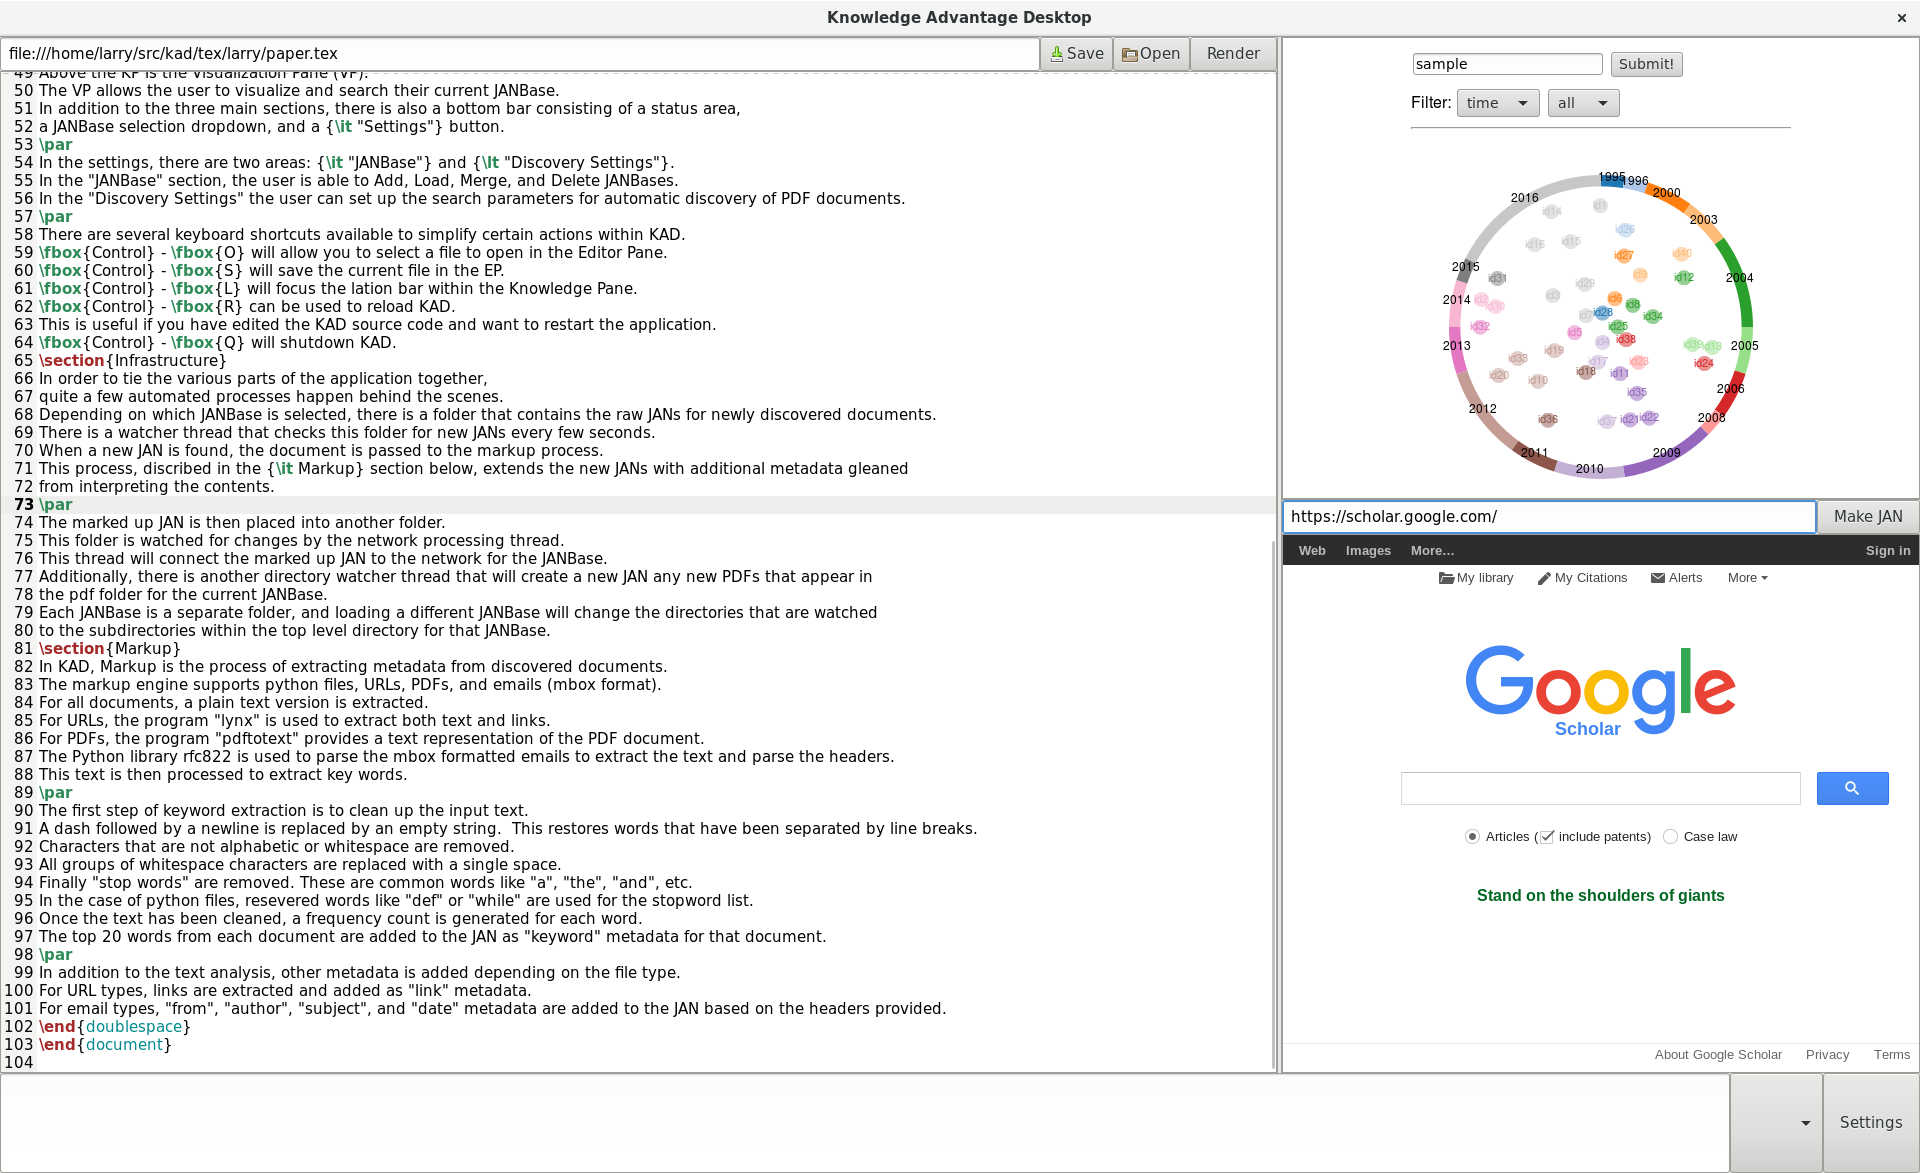
\includegraphics[width=6in]{images/kad-overview.png}\\
The KAD interface has three main sections.
On the left is the Editor Pane (EP).
The EP is intended for content production.
It allows you to edit any text file, from programming source code to TeX markup.
In the case of TeX markup, there is a {\it "Render"} button that will generate a PDF document.
This PDF will be shown in the lower left pane, which we call the Knowledge Pane (KP).
\par
The KP will show both web sites as well as PDF documents.
At the top of the KP is the location bar, which allows you to directly navigate to any URL or PDF file.
When browsing web sites, if a PDF link is selected, the PDF is automatically downloaded and displayed
in the KP.
If the current document being shown in the KP does not have an existing JAN, there will be a
{\it "Make JAN"} button displayed.
This button allows the user to create a JAN from the window's current contents,
facilitating manual discovery in addition to the automated discovery provided by the web crawler.
\par
Above the KP is the Visualization Pane (VP).
The VP allows the user to visualize and search their current JANBase.
In addition to the three main sections, there is also a bottom bar consisting of a status area,
a JANBase selection dropdown, and a {\it "Settings"} button.
\par
In the settings, there are two areas: {\it "JANBase"} and {\lt "Discovery Settings"}.
In the "JANBase" section, the user is able to Add, Load, Merge, and Delete JANBases.
In the "Discovery Settings" the user can set up the search parameters for automatic discovery of PDF documents.
\par
There are several keyboard shortcuts available to simplify certain actions within KAD.
\fbox{Control} - \fbox{O} will allow you to select a file to open in the Editor Pane.
\fbox{Control} - \fbox{S} will save the current file in the EP.
\fbox{Control} - \fbox{L} will focus the location bar within the Knowledge Pane.
\fbox{Control} - \fbox{R} can be used to reload KAD.
This is useful if you have edited the KAD source code and want to restart the application.
\fbox{Control} - \fbox{Q} will shutdown KAD.
\section{Infrastructure}
In order to tie the various parts of the application together,
quite a few automated processes happen behind the scenes.
Depending on which JANBase is selected, there is a folder that contains the raw JANs for newly discovered documents.
There is a watcher thread that checks this folder for new JANs every few seconds.
When a new JAN is found, the document is passed to the markup process.
This process, described in the {\it Markup} section below, extends the new JANs with additional metadata gleaned
from interpreting the contents.
\par
The marked up JAN is then placed into another folder.
This folder is watched for changes by the network processing thread.
This thread will connect the marked up JAN to the network for the JANBase.
Additionally, there is another directory watcher thread that will create a new JAN any new PDFs that appear in
the PDF folder for the current JANBase.
Each JANBase is a separate folder, and loading a different JANBase will change the directories that are watched
to the subdirectories within the top level directory for that JANBase. 
\section{Markup}
In KAD, Markup is the process of extracting metadata from discovered documents.
The markup engine supports python files, URLs, PDFs, and emails (mbox format).
For all documents, a plain text version is extracted.
For URLs, the program "lynx" is used to extract both text and links.
For PDFs, the program "pdftotext" provides a text representation of the PDF document.
The Python library rfc822 is used to parse the mbox formatted emails to extract the text and parse the headers.
This text is then processed to extract key words.
\par
The first step of keyword extraction is to clean up the input text.
A dash followed by a newline is replaced by an empty string.  This restores words that have been separated by line breaks.
Characters that are not alphabetic or whitespace are removed.
All groups of whitespace characters are replaced with a single space.
Finally "stop words" are removed. These are common words like "a", "the", "and", etc.
In the case of python files, reserved words like "def" or "while" are used for the stopword list.
Once the text has been cleaned, a frequency count is generated for each word.
The top 20 words from each document are added to the JAN as "keyword" metadata for that document.
\par
In addition to the text analysis, other metadata is added depending on the file type.
For URL types, links are extracted and added as "link" metadata.
For email types, "from", "author", "subject", and "date" metadata are added to the JAN based on the headers provided.
\par
As future work, there are a few things that could be done to improve the markup process beyond simple frequency analysis.
In addition to more advanced word and phrase frequency analysis techniques,
there is likely room to leverage deep learning models in order to intelligently parse unstructured data.
For example, the problem of identifying the authors and extracting the abstract from an arbitrary PDF file is quite difficult.
Beyond the high level classification of separating book chapters from journal articles and theses and dissertations, there are a multitude of possible formats
that would make a heuristics based approach very quickly become untenable.
Depending on the target domain, there will be different pieces of relevant information that can be extracted given enough examples.
Ideally, it would be possible to create a generic tool that could be trained for whatever domain you wanted to apply it to.
\end{doublespace}
\end{document}
